% !Mode:: "TeX:UTF-8:Main"
% arara: pdflatex
% arara: convert: {density: 160, otheroptions: -dispose previous -delay 20 -loop 1, format: gif}
% xarara: showfile: {format: gif}
\documentclass{article}
\usepackage[utf8]{inputenc} %probably not needed ...
\usepackage[T1]{fontenc}
\usepackage{geometry}
\geometry{papersize={128mm,96mm},margin=0.5cm} %\textwidth=11.8, \textheight=8.6
\usepackage[x11names,svgnames]{xcolor}
\usepackage{tikzducks}
\usetikzlibrary{shapes.geometric}
\pagestyle{empty}
\parindent=0pt
\usepackage{animate}
\usepackage{eso-pic}
\usepackage{xfp}
\definecolor{mggreen}{RGB}{37,166,89}
\definecolor{swordcolorlight}{RGB}{230,230,230}
\colorlet{swordcolordark}{black}

\tikzset{
piratehat/.pic={
\begin{scope}[y=0.80pt, x=0.80pt,yshift=20,xshift=-20.3, yscale=-0.1400000, xscale=0.1400000, inner sep=0pt, outer sep=0pt]
\path[fill=black,even odd rule,line width=0.469pt] (33.5791,125.7356) ..
  controls (38.7275,127.1585) and (47.7673,129.5133) .. (56.7180,132.1614) ..
  controls (81.3596,139.4459) and (96.9942,134.6382) .. (111.1091,113.1908) ..
  controls (119.0669,101.1023) and (125.8950,88.0413) .. (131.5460,74.7035) ..
  controls (146.9618,38.3007) and (176.0263,22.4426) .. (213.3558,21.0937) ..
  controls (253.2073,19.6514) and (285.5832,34.1323) .. (304.3168,71.7786) ..
  controls (309.7925,82.7809) and (314.7338,94.0665) .. (320.5919,104.8577) ..
  controls (336.0792,133.3866) and (352.7267,140.2324) .. (383.9829,131.8418) ..
  controls (392.6861,129.5028) and (401.4673,126.8688) .. (410.3694,126.0101) ..
  controls (419.4714,125.1333) and (422.3998,130.1802) .. (417.9330,138.1286) ..
  controls (415.1236,143.1291) and (411.2380,147.6523) .. (407.2615,151.8429) ..
  controls (385.1788,175.0991) and (363.0258,198.2938) .. (340.5426,221.1612) ..
  controls (338.5203,223.2175) and (333.8358,223.8251) .. (330.6323,223.3712) ..
  controls (298.6447,218.8421) and (266.7967,213.2275) .. (234.7358,209.3501) ..
  controls (197.8485,204.8909) and (161.7547,212.2697) .. (126.0833,220.4421) ..
  controls (108.6387,224.4392) and (96.2798,224.1025) .. (83.7848,207.3043) ..
  controls (68.8687,187.2499) and (48.5597,171.2258) .. (30.7586,153.2875) ..
  controls (26.9169,149.4177) and (23.2249,145.1678) .. (20.4636,140.5016) ..
  controls (13.8489,129.3262) and (16.3457,125.4887) .. (33.5791,125.7356) --
  cycle;
\path[fill=white,even odd rule,line width=0.469pt] (244.2824,154.3362) ..
  controls (241.1862,166.6974) and (235.6431,178.2616) .. (220.7610,178.0534) ..
  controls (205.7001,177.8393) and (197.0262,167.9074) .. (191.6549,151.2857) ..
  controls (187.6456,156.4840) and (184.6755,160.0470) .. (182.0567,163.8523) ..
  controls (180.8034,165.6757) and (180.6960,168.4505) .. (179.2081,169.9156) ..
  controls (177.0738,172.0153) and (174.0175,174.7197) .. (171.6063,174.4921) ..
  controls (169.7952,174.3226) and (167.9189,170.1174) .. (166.9277,167.3965) ..
  controls (166.0837,165.0839) and (166.4597,162.3244) .. (164.3201,160.9532) ..
  controls (161.3571,156.5244) and (158.3929,152.0980) .. (155.4298,147.6699) ..
  controls (160.9852,146.5784) and (166.6016,145.7133) .. (172.0808,144.3227) ..
  controls (177.1007,143.0511) and (182.4902,141.9813) .. (186.6344,139.2077) ..
  controls (188.1042,138.2236) and (187.1160,132.2353) .. (186.0069,128.9550) ..
  controls (181.2667,114.9556) and (176.5541,112.5761) .. (162.1172,113.8330) ..
  controls (158.3207,114.1621) and (154.2463,111.2454) .. (150.2996,109.8166) ..
  controls (152.3301,106.6184) and (154.3506,103.4131) .. (156.3911,100.2207) ..
  controls (157.9272,97.8219) and (159.6046,95.5046) .. (161.0116,93.0337) ..
  controls (163.0421,89.4689) and (164.8808,85.7973) .. (166.8040,82.1750) ..
  controls (169.9876,85.5087) and (173.4526,88.6208) .. (176.2779,92.2354) ..
  controls (179.0655,95.8014) and (181.2075,99.8735) .. (184.0643,104.4149) ..
  controls (206.7822,76.5205) and (232.5452,76.4208) .. (252.4706,104.4413) ..
  controls (255.4337,100.6471) and (258.1592,97.4970) .. (260.4665,94.0683) ..
  controls (261.6958,92.2389) and (261.6642,89.3175) .. (263.1668,87.9750) ..
  controls (265.6096,85.7932) and (268.8454,84.5041) .. (271.7462,82.8384) ..
  controls (273.2149,85.4659) and (274.7374,88.0648) .. (276.1357,90.7316) ..
  controls (277.9052,94.1040) and (279.3855,97.6448) .. (281.3439,100.9029) ..
  controls (283.1773,103.9568) and (285.4706,106.7345) .. (287.5626,109.6366) ..
  controls (283.2735,111.1269) and (279.0688,112.9838) .. (274.6718,114.0102) ..
  controls (269.3562,115.2483) and (261.9914,113.9081) .. (258.8911,117.0342) ..
  controls (253.6454,122.3187) and (251.0530,130.2365) .. (247.4126,136.9251) ..
  controls (255.5322,143.9028) and (262.8741,147.3180) .. (272.4800,144.7092) ..
  controls (275.0882,144.0025) and (278.5175,146.3116) .. (281.5679,147.2377) ..
  controls (280.1234,150.1473) and (278.7668,153.1039) .. (277.2143,155.9549) ..
  controls (275.1017,159.8323) and (272.8841,163.6540) .. (270.6307,167.4505) ..
  controls (269.1521,169.9408) and (267.5287,172.3432) .. (265.9703,174.7842) ..
  controls (263.3439,172.9379) and (259.8219,171.6423) .. (258.2712,169.1273) ..
  controls (254.7146,163.3696) and (254.3504,155.0670) .. (244.2824,154.3362) --
  cycle;
\path[fill=black,even odd rule,line width=0.469pt] (215.4097,115.6635) ..
  controls (215.5177,122.3321) and (209.5441,127.8195) .. (201.9928,127.5767) ..
  controls (194.4374,127.3321) and (191.4086,122.0436) .. (190.5840,115.5761) ..
  controls (189.8808,110.0530) and (197.1494,102.9140) .. (202.7681,102.7803) ..
  controls (209.8807,102.6108) and (215.2883,108.1198) .. (215.4097,115.6635) --
  cycle;
\path[fill=black,even odd rule,line width=0.469pt] (235.9065,127.7679) ..
  controls (227.2032,127.8717) and (219.9546,121.5849) .. (222.0349,115.0459) ..
  controls (223.5493,110.2858) and (229.0965,104.4817) .. (233.7329,103.5492) ..
  controls (241.9416,101.9011) and (245.5363,109.1544) .. (246.0965,116.3750) ..
  controls (246.6918,124.1040) and (240.7581,126.5245) .. (235.9065,127.7679) --
  cycle;
\path[fill=black,even odd rule,line width=0.469pt] (218.4502,126.4553) ..
  controls (221.4250,131.4781) and (223.4555,134.9116) .. (226.0138,139.2289) ..
  controls (220.6643,139.2289) and (216.6637,139.2289) .. (211.4831,139.2289) ..
  controls (213.7640,135.0465) and (215.6731,131.5456) .. (218.4502,126.4553) --
  cycle;
  \end{scope}
}
}

\tikzset{picpirateswordhandle/.style={fill=#1,draw=#1}}
\tikzset{picpirateswordblade/.style={fill=#1,draw=#1}}

\tikzset{swordhandle/.style={picpirateswordhandle/.style={fill=#1,draw=#1}}}
\tikzset{swordblade/.style   ={picpirateswordblade/.style={fill=#1,draw=#1}}}

\tikzset{ piratesword/.pic=
{
 \begin{scope}[y=0.80pt, x=0.80pt, yscale=-0.1000000, xscale=0.1000000, inner sep=0pt, outer sep=0pt]
  \begin{scope}[cm={{1.25,0.0,0.0,1.25,(-95.12185,-232.5044)}}]
   \path[picpirateswordhandle=swordcolordark,line width=0.075pt] (73.6300,68.7000) .. controls
      (77.3200,65.4400) and (83.1600,66.2500) .. (86.7600,69.2500) .. controls
      (92.0400,73.4500) and (94.2300,80.2500) .. (95.5100,86.6300) .. controls
      (99.6500,87.3200) and (103.8400,86.4000) .. (107.9800,86.8700) .. controls
      (111.6000,87.7600) and (115.2700,92.7800) .. (111.9200,95.9500) .. controls
      (108.8300,98.5600) and (104.7100,99.3600) .. (101.1600,101.1700) .. controls
      (106.2400,119.4400) and (115.0200,136.4200) .. (120.5600,154.5500) .. controls
      (123.3600,163.8600) and (126.4500,173.1300) .. (130.6700,181.9100) .. controls
      (136.4500,181.4600) and (141.1900,177.3500) .. (146.9900,177.1000) .. controls
      (150.2500,177.0100) and (152.9900,179.8400) .. (153.2400,183.0100) .. controls
      (154.3800,193.0600) and (148.6100,202.3900) .. (141.2900,208.7800) .. controls
      (137.0100,211.2700) and (132.2600,212.8300) .. (127.7400,214.8200) .. controls
      (121.8700,217.0900) and (116.2000,220.5000) .. (109.7100,220.4400) .. controls
      (94.7800,221.6300) and (79.6200,216.3500) .. (68.0700,206.9300) .. controls
      (60.1100,200.3000) and (54.4500,191.4100) .. (49.7700,182.2800) .. controls
      (46.5300,175.6200) and (43.6500,168.5700) .. (43.2500,161.0900) .. controls
      (42.4100,146.7800) and (44.7500,131.8100) .. (52.6300,119.5900) .. controls
      (57.8900,110.6800) and (65.4000,103.4300) .. (73.1900,96.7600) .. controls
      (72.0900,89.6700) and (66.9400,83.3700) .. (67.9500,75.9500) .. controls
      (68.1400,72.5100) and (71.3100,70.7100) .. (73.6300,68.7000)(60.2400,128.1600)
      .. controls (54.1400,149.5700) and (64.1600,174.4000) .. (83.4100,185.5800) ..
      controls (90.8200,189.9700) and (100.0700,190.3200) .. (108.0600,187.3100) ..
      controls (104.5300,178.0900) and (100.9700,168.8700) .. (97.2000,159.7400) ..
      controls (93.9300,153.6000) and (92.5100,146.7400) .. (89.8900,140.3300) ..
      controls (85.7700,129.9000) and (83.7000,118.5700) .. (77.5900,109.0100) ..
      controls (68.6100,111.2900) and (62.7900,119.7100) .. (60.2400,128.1600) --
      cycle;
    \path[picpirateswordblade=swordcolorlight,line width=0.075pt] (127.7400,214.8200) ..
      controls (132.2600,212.8300) and (137.0100,211.2700) .. (141.2900,208.7800) ..
      controls (141.8900,211.8700) and (142.8400,214.9000) .. (144.3200,217.7000) ..
      controls (147.6000,224.0500) and (150.5900,230.5700) .. (154.3000,236.6900) ..
      controls (164.9200,253.3200) and (176.3900,269.5800) .. (190.6100,283.3800) ..
      controls (197.6900,291.1300) and (206.1100,297.4800) .. (215.0000,303.0200) ..
      controls (239.1100,320.3900) and (266.0100,334.8900) .. (295.4200,340.6500) ..
      controls (304.1800,342.6200) and (313.1000,343.7400) .. (322.0700,344.1100) ..
      controls (326.5000,344.4800) and (331.6600,344.5900) .. (334.8700,348.1400) ..
      controls (338.1900,351.9900) and (339.1700,357.1800) .. (341.3800,361.6700) ..
      controls (346.7200,372.9600) and (353.5800,383.6700) .. (362.6900,392.3100) ..
      controls (366.6500,396.7200) and (371.8700,399.8100) .. (375.6600,404.3700) ..
      controls (377.7100,406.6200) and (376.6700,410.9400) .. (373.6500,411.7200) ..
      controls (369.8700,412.7700) and (365.9100,412.0500) .. (362.0800,411.7600) ..
      controls (330.2500,408.7000) and (298.9400,401.1300) .. (269.0100,389.9600) ..
      controls (257.7500,385.1700) and (246.5600,380.1600) .. (235.8600,374.2000) ..
      controls (220.6200,366.4100) and (206.9400,356.0300) .. (193.5300,345.4700) ..
      controls (181.8600,336.1500) and (172.8700,324.1100) .. (162.8000,313.1900) ..
      controls (153.8100,303.4400) and (146.9200,292.0000) .. (140.4800,280.4700) ..
      controls (131.7100,265.7300) and (126.0900,249.4000) .. (120.8500,233.1500) ..
      controls (119.4200,229.2300) and (119.2000,224.7400) .. (116.6600,221.3100) ..
      controls (114.4100,220.6100) and (112.0400,220.5700) .. (109.7100,220.4400) ..
      controls (116.2000,220.5000) and (121.8700,217.0900) .. (127.7400,214.8200) --
      cycle;
  \end{scope}
\end{scope}
}
}


\tikzset{eyepatch/.pic={
    %\fill[\duck@sunglasses,rotate=-17] (0.42,1.8) rectangle (0.8,1.84);
	%\fill[\duck@sunglasses,rotate=-17] (0.12,1.8) rectangle (0.22,1.84);
	\fill[black] (0.82,1.6275) circle [x radius=0.14,y radius=0.2,rotate=20];
    \draw[bend left](0.83,1.6275) to (.75,2.2);
    \draw[bend right](0.83,1.6275) to (1.2,1.15);
%	\fill[black,rotate=-20] (-0.06,1.74) circle (0.13);				
}
}


\tikzset{duckparrot/.pic={
    \path(0,0)--++(1,0);
    \begin{scope}[scale=0.2,xshift=40,yshift=20,transform shape]
    \duck[name=parrot]body=yellow];
    \draw (parrot-head) pic [rotate=-20] {piratehat};
    \end{scope}			
}
}

\tikzset{cross/.pic={
     \begin{scope}[xshift=10.3cm,yshift=-7.2cm]
     \begin{scope}[y=0.80pt, x=0.80pt, yscale=1.000000, xscale=1.000000, inner sep=0pt, outer sep=0pt,rotate=90]
      \path[fill=white] (305.9800,336.9390) .. controls (303.5570,332.9030) and
        (298.3170,331.5890) .. (294.2720,334.0210) -- (256.0000,356.9830) --
        (217.7280,334.0200) .. controls (213.6750,331.5880) and (208.4440,332.9020) ..
        (206.0200,336.9380) .. controls (203.5880,340.9830) and (204.9020,346.2220) ..
        (208.9380,348.6460) -- (239.4190,366.9330) -- (208.9380,385.2200) .. controls
        (204.9020,387.6430) and (203.5880,392.8830) .. (206.0200,396.9280) .. controls
        (207.6160,399.5900) and (210.4400,401.0670) .. (213.3420,401.0670) .. controls
        (214.8350,401.0670) and (216.3460,400.6740) .. (217.7280,399.8470) --
        (256.0000,376.8830) -- (294.2720,399.8460) .. controls (295.6460,400.6740) and
        (297.1650,401.0660) .. (298.6580,401.0660) .. controls (301.5590,401.0660) and
        (304.3840,399.5900) .. (305.9800,396.9270) .. controls (308.4120,392.8820) and
        (307.0980,387.6430) .. (303.0620,385.2190) -- (272.5810,366.9320) --
        (303.0620,348.6450) .. controls (307.0980,346.2230) and (308.4120,340.9830) ..
        (305.9800,336.9390) -- cycle;
       \end{scope}
      \end{scope}
     }}
\begin{document}
\AddToShipoutPictureBG{%
 \AtPageLowerLeft{%
 
\begin{tikzpicture}[overlay,remember picture]
 \fill[PeachPuff2] (0,0) rectangle (\paperwidth,\paperheight);
 \end{tikzpicture}}}

\foreach\x in {10,20,...,360}
{
\begin{tikzpicture}[]
\path[use as bounding box] (0,0) rectangle (\textwidth,\textheight);

\begin{scope}[xshift=1cm,yshift=0cm]
\begin{scope}[xshift=1cm,yshift=2cm,xscale=-1,transform shape]
{\duck[name=main,tshirt=red,stripes={\stripes},body=DarkGoldenrod,shorthair=Maroon]}
\draw(main-head) pic [rotate=-20]{piratehat};
\pic{eyepatch};
\draw (main-wing) pic{duckparrot};
\draw (main-wing) pic [swordhandle=SlateGray,swordblade=Silver,rotate=\x] {piratesword};
\end{scope}

\begin{scope}[xshift=8cm,yshift=6cm]
\duck[tshirt=red,stripes={\stripes},longhair=red!50!Maroon,body=AntiqueWhite2!50!Goldenrod1]
\draw(head) pic [rotate=-20]{piratehat};
\pic{eyepatch};
\draw(wing) pic [swordhandle=SlateGray,swordblade=Silver,rotate=\x+30] {piratesword};
\end{scope}

\begin{scope}[xshift=7.2cm,yshift=3.6cm,scale=0.6,transform shape]
\duck[tshirt=red,stripes={\stripes},shorthair=brown]
\draw(head) pic [rotate=-20]{piratehat};
\pic{eyepatch};
\draw(wing) pic[swordhandle=SlateGray,swordblade=Silver,rotate=\x+70] {piratesword};
\end{scope}



\begin{scope}[xshift=7cm,yshift=2cm,scale=0.6,transform shape]
\duck[tshirt=red,stripes={\stripes},shorthair=brown]
\draw(head) pic [rotate=-20]{piratehat};
\pic{eyepatch};
\draw(wing) pic[swordhandle=SlateGray,swordblade=Silver,rotate=\x+20] {piratesword};
\end{scope}


\begin{scope}[xshift=6.3cm,yshift=5.4cm,scale=0.6,transform shape]
\duck[tshirt=red,stripes={\stripes},shorthair=brown]
\draw(head) pic [rotate=-20]{piratehat};
\pic{eyepatch};
\draw(wing) pic[swordhandle=SlateGray,swordblade=Silver,rotate=\x+110] {piratesword};
\end{scope}

\begin{scope}[xshift=5.8cm,yshift=7.3cm,scale=0.6,transform shape]
\duck[tshirt=red,stripes={\stripes},shorthair=brown]
\draw(head) pic [rotate=-20]{piratehat};
\pic{eyepatch};
\draw(wing) pic[swordhandle=SlateGray,swordblade=Silver,rotate=\x+210] {piratesword};
\end{scope}

\begin{scope}[xshift=8cm,yshift=1.3cm,scale=0.6,transform shape]
\duck[tshirt=red,stripes={\stripes},shorthair=brown]
\draw(head) pic [rotate=-20]{piratehat};
\pic{eyepatch};
\draw(wing) pic[swordhandle=SlateGray,swordblade=Silver,rotate=\x+80] {piratesword};
\end{scope}

\begin{scope}[xshift=9.6cm,yshift=3.3cm,scale=0.6,transform shape]
\duck[tshirt=red,stripes={\stripes},shorthair=brown]
\draw(head) pic [rotate=-20]{piratehat};
\pic{eyepatch};
\draw(wing) pic[swordhandle=SlateGray,swordblade=Silver,rotate=\x+150] {piratesword};
\end{scope}

\begin{scope}[xshift=8.2cm,yshift=0cm,scale=0.6,transform shape]
\duck[tshirt=red,stripes={\stripes},shorthair=brown]
\draw(head) pic [rotate=-20]{piratehat};
\pic{eyepatch};
\draw(wing) pic[swordhandle=SlateGray,swordblade=Silver,rotate=\x+270] {piratesword};
\end{scope}



\begin{scope}[xshift=3cm,yshift=0cm,scale=0.6,xscale=-1,transform shape]
\duck[tshirt=red,stripes={\stripes},shorthair=brown]
\draw(head) pic [rotate=-20]{piratehat};
\pic{eyepatch};
\draw(wing) pic[swordhandle=SlateGray,swordblade=Silver,rotate=\x+145] {piratesword};
\end{scope}

\begin{scope}[xshift=1cm,yshift=5cm,scale=0.6,xscale=-1,transform shape]
\duck[tshirt=red,stripes={\stripes},shorthair=brown]
\draw(head) pic [rotate=-20]{piratehat};
\pic{eyepatch};
\draw(wing) pic[swordhandle=SlateGray,swordblade=Silver,rotate=\x+55] {piratesword};
\end{scope}

\begin{scope}[xshift=2cm,yshift=7cm,scale=0.6,xscale=-1,transform shape]
\duck[tshirt=red,stripes={\stripes},shorthair=brown]
\draw(head) pic [rotate=-20]{piratehat};
\pic{eyepatch};
\draw(wing) pic[swordhandle=SlateGray,swordblade=Silver,rotate=\x+100] {piratesword};
\end{scope}

\begin{scope}[xshift=3cm,yshift=6.5cm,scale=0.6,xscale=-1,transform shape]
\duck[tshirt=red,stripes={\stripes},shorthair=brown]
\draw(head) pic [rotate=-20]{piratehat};
\pic{eyepatch};
\draw(wing) pic[swordhandle=SlateGray,swordblade=Silver,rotate=\x] {piratesword};
\end{scope}

\begin{scope}[xshift=3.2cm,yshift=4.5cm,scale=0.6,xscale=-1,transform shape]
\duck[tshirt=red,stripes={\stripes},shorthair=brown]
\draw(head) pic [rotate=-20]{piratehat};
\pic{eyepatch};
\draw(wing) pic[swordhandle=SlateGray,swordblade=Silver,rotate=\x+130] {piratesword};
\end{scope}


\begin{scope}[xshift=2.5cm,yshift=2.5cm,scale=0.6,xscale=-1,transform shape]
\duck[tshirt=red,stripes={\stripes},shorthair=brown]
\draw(head) pic [rotate=-20]{piratehat};
\pic{eyepatch};
\draw(wing) pic[swordhandle=SlateGray,swordblade=Silver,rotate=\x+170] {piratesword};
\end{scope}


\fill[Burlywood4] (4,0) --++ (-0.5,5) --++ (0.5,2) --++ (2,0)--++ (0.5,-2) --++(-0.5,-5) --cycle;
\coordinate (crosscenter) at (5,5.5);

\begin{scope}[scale=0.5]
\draw[line width=3mm,white] ([yshift=-3cm]crosscenter)--++(0,3.8)
                            ([xshift=-0.8cm]crosscenter)--++(1.6,0);
\end{scope}

\begin{scope}[yshift=8.88cm,xshift=4.1cm]
 \begin{scope}[y=0.80pt, x=0.80pt, yscale=-0.1300000, xscale=0.1300000, inner sep=0pt, outer sep=0pt,transform shape
    ]% g16
      \path[draw=brown,fill=black] (378.8290,196.9580) -- (319.5480,171.5630) .. controls (308.1470,165.8710)
        and (307.2000,155.3500) .. (307.2000,145.0670) -- (307.2000,102.4000) ..
        controls (316.6040,102.4000) and (324.2670,94.7460) .. (324.2670,85.3330) --
        (324.2670,51.2000) .. controls (324.2670,41.7880) and (316.6040,34.1330) ..
        (307.2000,34.1330) -- (290.1330,34.1330) -- (290.1330,8.5330) .. controls
        (290.1330,3.8230) and (286.3190,0.0000) .. (281.6000,0.0000) --
        (230.4000,0.0000) .. controls (225.6810,0.0000) and (221.8670,3.8230) ..
        (221.8670,8.5330) -- (221.8670,34.1330) -- (204.8000,34.1330) .. controls
        (195.3880,34.1330) and (187.7330,41.7870) .. (187.7330,51.2000) --
        (187.7330,85.3330) .. controls (187.7330,94.7450) and (195.3870,102.4000) ..
        (204.8000,102.4000) -- (204.8000,145.0670) .. controls (204.8000,155.3500) and
        (203.8530,165.8710) .. (192.9050,171.3580) -- (132.7190,197.1630) .. controls
        (113.1690,206.9420) and (102.4000,224.8020) .. (102.4000,247.4670) --
        (102.4000,469.3340) .. controls (102.4000,492.8600) and (121.5400,512.0010) ..
        (145.0670,512.0010) -- (366.9340,512.0010) .. controls (390.4600,512.0010) and
        (409.6010,492.8610) .. (409.6010,469.3340) -- (409.6010,247.4670) .. controls
        (409.6000,224.8020) and (398.8310,206.9420) .. (378.8290,196.9580) --
        cycle;

        \path[fill=brown!60!black]
        (238.9330,17.0670) -- (273.0660,17.0670) -- (273.0660,34.1340) --
        (238.9330,34.1340) -- (238.9330,17.0670) -- cycle;

        \path (175,367)pic{cross}--++ (80,0) pic {cross}--++(80,0) pic {cross};
 \end{scope}
 \end{scope}
 \end{scope}
\end{tikzpicture}\newpage}

\end{document}
%test rotate sword: ~220-300
\newpage
\raggedright
\foreach\x in {10,20,...,360}
{
\begin{tikzpicture}
\duck[tshirt=red,stripes={\stripes},longhair=red!50!Maroon,body=AntiqueWhite2!50!Goldenrod1]
\draw(head) pic [rotate=-20]{piratehat};
\pic{eyepatch};
\draw[overlay](wing) pic [swordhandle=SlateGray,swordblade=Silver,rotate=\x] {piratesword};
\path(0,0)--++(0,-0.5);
\end{tikzpicture}\newpage
}




\end{document}

xxx\fbox{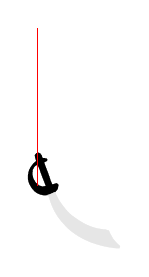
\begin{tikzpicture}[]
\draw(0,0) --++ (0,2);
\draw(0,0) pic {piratesword};
\draw[red](0,0) --++ (0,2);
\end{tikzpicture}}



xxx\fbox{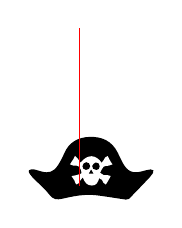
\begin{tikzpicture}[]
\draw(0,0) --++ (0,2);
\draw(0,0) pic {piratehat};
\draw[red](0,0) --++ (0,2);
\end{tikzpicture}}
